%--------------------------------------------------
\section{Proceso ajustado}


Con el desarrollo del sistema, un paciente, previamente registrado en el mismo, al presentar la necesidad de ser atendido por un médico, tendrá la opción de realizar una cita en línea donde el sistema le mostrará al paciente los horarios disponibles y no disponibles de cada día, separando cada horario para cada consultorio con su respectivo médico. Si el paciente agenda una cita en algunos de estos horarios disponibles, entonces una cita se generará para dicho horario y consultorio.\\ 

Hecho esto, el paciente debe de presentarse en la clínica 10 minutos antes de la hora de su cita para poder realizar el pago de la consulta con el cajero, para que el cajero pueda entonces realizar el registro de dicho pago y habilitar la cita.\\

Al ser atendido el paciente, el médico realiza el diagnóstico y tratamiento para la enfermedad del paciente en caso de existir dicha enfermedad, y el médico crea o actualiza el expediente del paciente con el diagnóstico y tratamiento.\\

Al finalizar la consulta, el paciente puede adquirir los medicamentos necesarios para el tratamiento en la farmacia de la clínica, donde el farmacéutico despacha los medicamentos, realiza el registro de la venta de medicamentos y el sistema actualiza el inventario de los mismos.\\

\subsection{Proceso de citas}
\begin{figure}[htbp!]
		\centering
			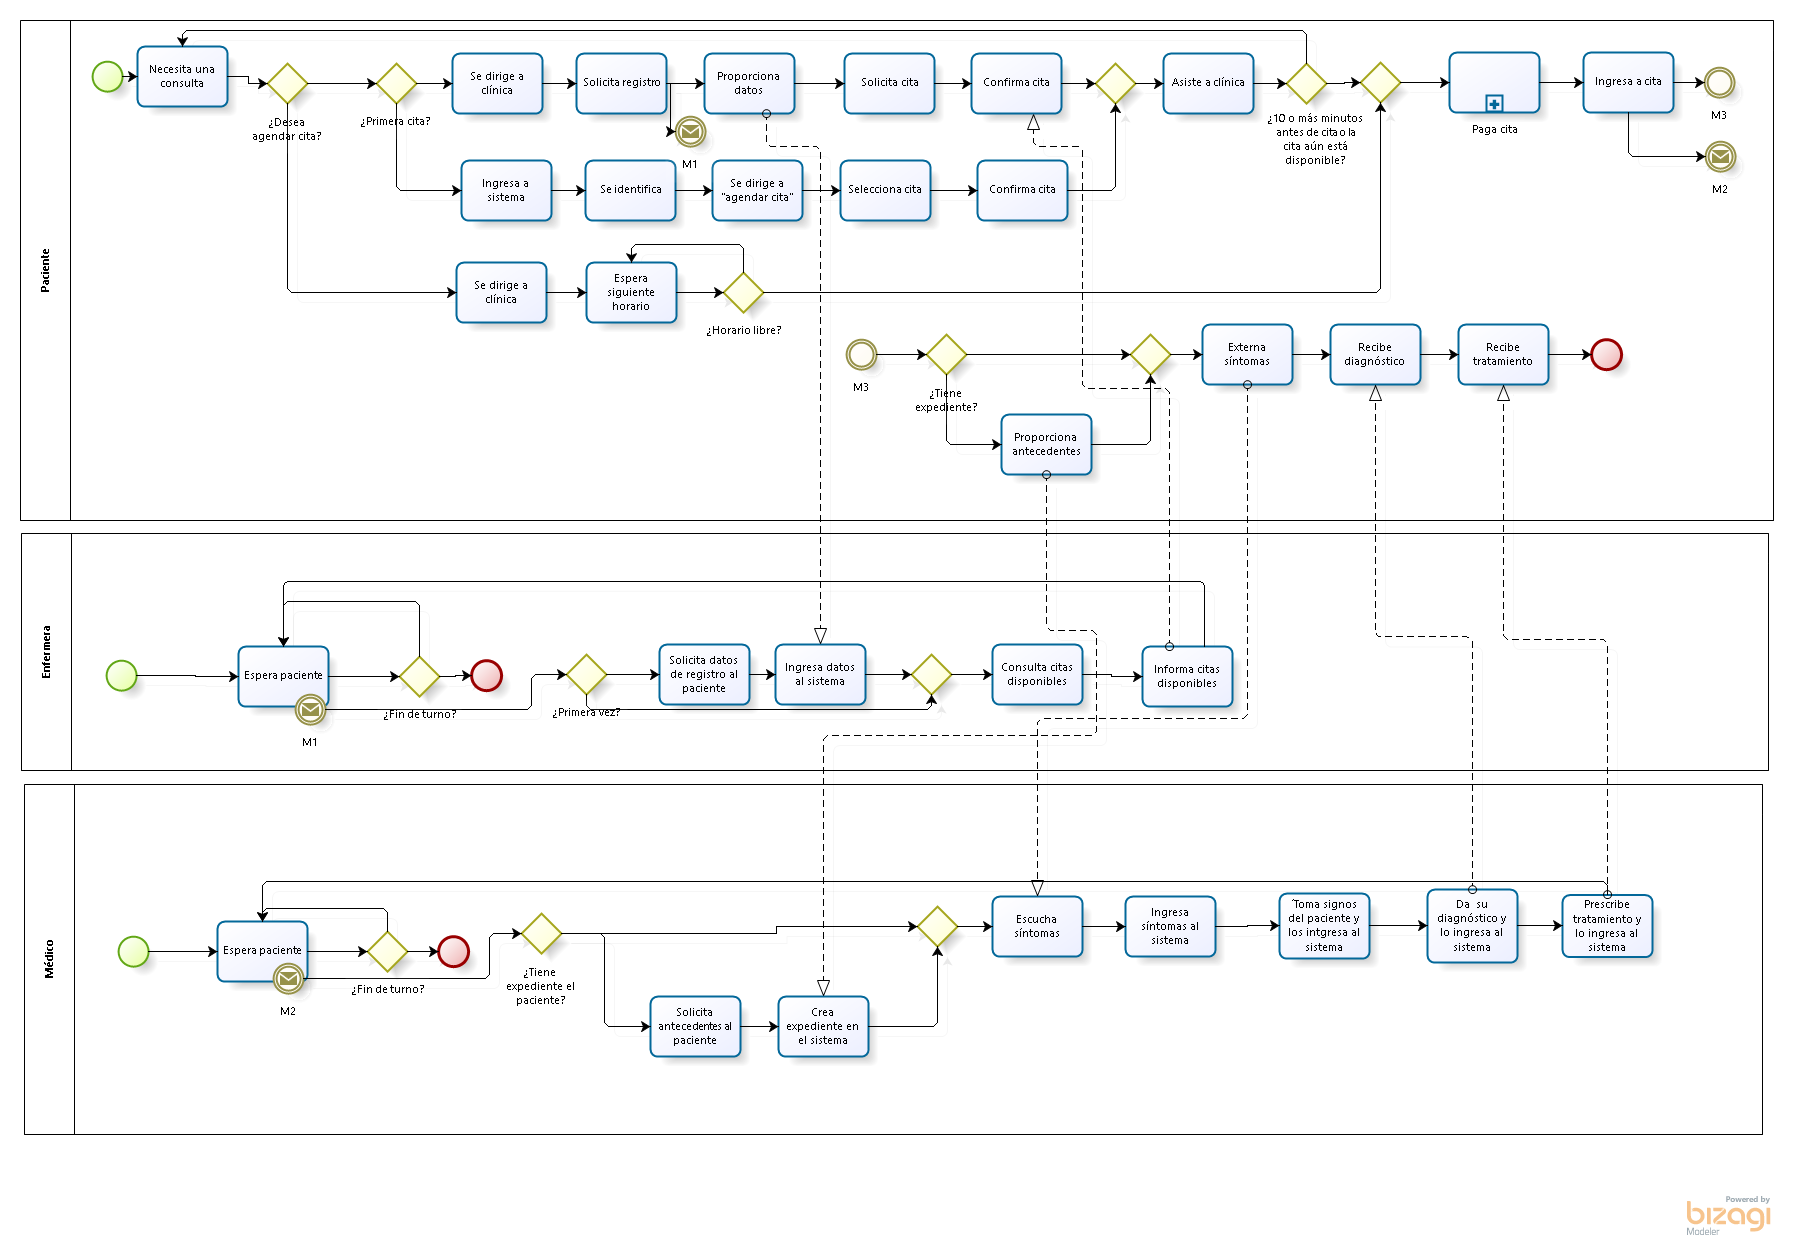
\includegraphics[width=1\textwidth]{images/procesos/consultas_new}
		\caption{Diagrama del proceso de citas.}
	\end{figure}
El paciente puede registrarse en línea o acudir personalmente a la clínica para que una enfermera lo registre. Asímismo, puede agendar una cita desde la aplicación o una enfermera puede hacerlo por él.\\
Al momento de pasar a consulta, el médico consulta el expediente del paciente desde la aplicación; en caso de que no exista el expediente se crea al momento, en dado caso el paciente informa al médico sus antecedentes médicos. El paciente informa al médico sus síntomas y el médico registra su diagnóstico y su correspondiente tratamiento en el sistema. El paciente posteriormente puede revisar la consulta ingresando al sistema con su cuenta de usuario.

\subsection{Proceso de cancelación de citas}
\begin{figure}[htbp!]
	\centering
	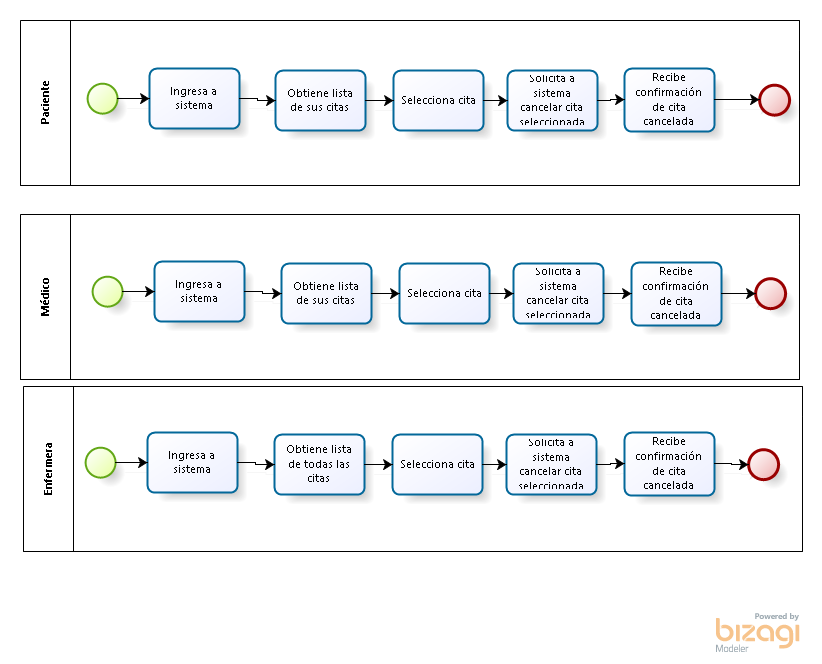
\includegraphics[width=0.7\textwidth]{images/procesos/cancelar_cita_new}
	\caption{Diagrama del proceso de la cancelación de citas.}
\end{figure}
El paciente si lo desea puede cancelar una cita agendada con antelación. Para ello se identifica en el sistema, consulta sus citas agendadas y cancela la cita que desee.\\
Por otro lado, la enfermera puede cancelar citas consultando las citas agendadas y seleccionando la cita que desea cancelar.\\
El médico también puede cancelar sus citas en caso de ser necesario, para ello consulta todas sus citas programadas y selecciona la cita que desea cancelar.

\subsection{Proceso de pago de citas}
\begin{figure}[htbp!]
		\centering
			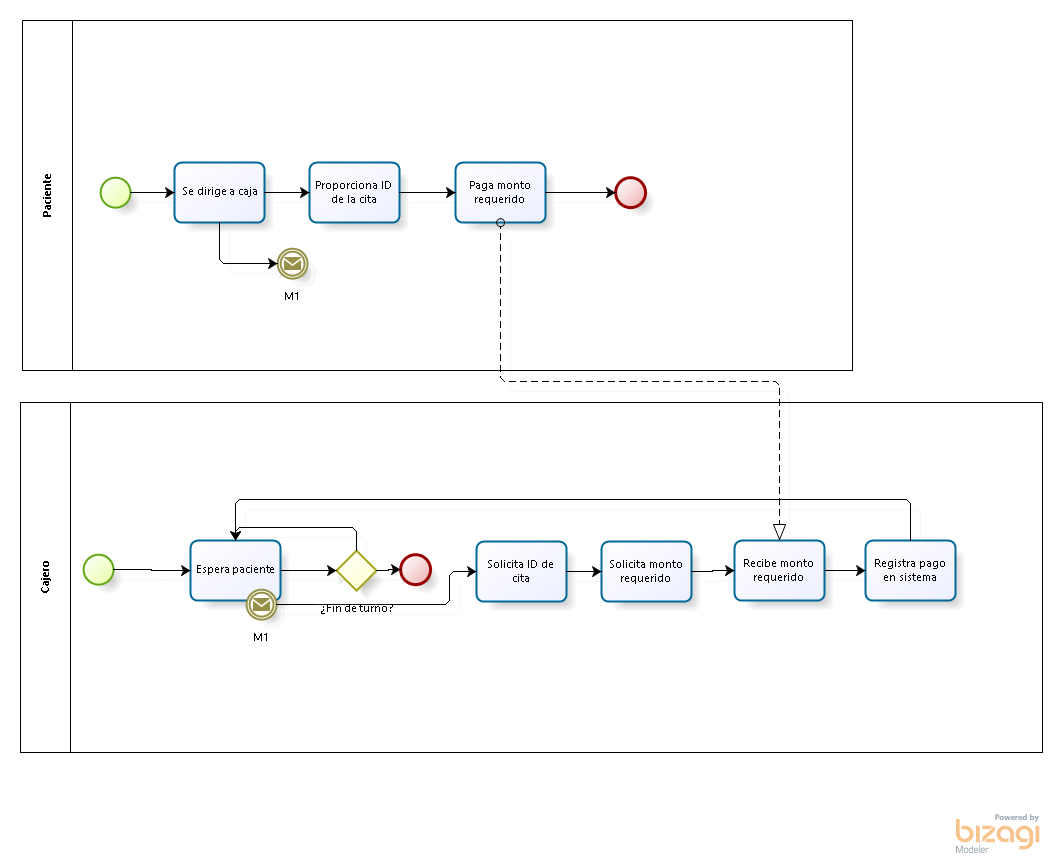
\includegraphics[width=0.7\textwidth]{images/procesos/pago_consulta_new}
		\caption{Diagrama del proceso de pago de citas.}
	\end{figure}
El paciente acude a la farmacia a realizar el pago de la cita, para ello proporciona al cajero la hora de la cita y el consultorio. El cajero ingresa la fecha de hoy, la hora de la cita y el consultorio en el sistema. Con ello se registra el pago de la cita y el paciente ya puede pasar a consulta.
    \subsection{Proceso de adquisición de medicamentos}
\begin{figure}[htbp!]
		\centering
			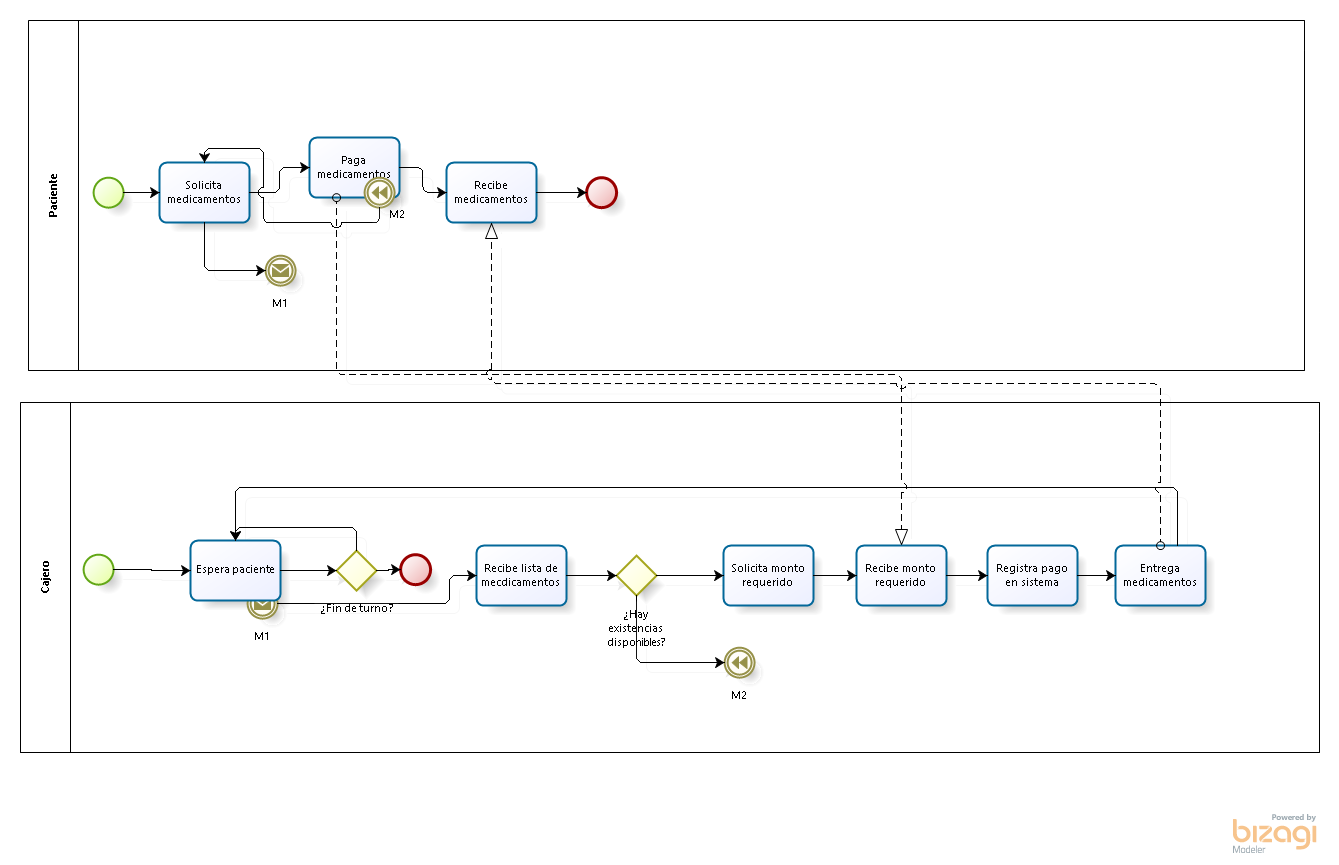
\includegraphics[width=0.7\textwidth]{images/procesos/medicamentos}
		\caption{Diagrama del proceso de adquisición de medicamentos.}
	\end{figure}
	El paciente acude a la farmacia e informa los medicamentos deseados al cajero. El cajero ingresa en el sistema los medicamentos disponibles en inventario, así como la cantidad a comprar. El cajero informa el monto al paciente y espera el pago. Por último registra la compra en el sistema y entrega los medicamentos al paciente.
\newpage
%--------------------------------------------------
\section{Procesos actuales}

% - - - - - - - - - - - - - - - - - - - - - - - - -
\subsection{Participantes}

\begin{itemize}
	\item \textbf{Paciente: }Es quien recibe los servicios médicos de la clínica. Debe asistir a la clínica o comunicarse vía telefónica para agendar una cita. Debe pagarla 10 minutos antes de su hora o podrá ser ocupada por otro paciente.
    \item \textbf{Enfermera: }Se encarga de la gestión de los horarios del consultorio. Es quien agenda las citas a los pacientes, y debe de proporcionar el expediente médico de los pacientes que se atenderán en el día al médico y si hay un paciente sin cita será la encargada de obtener su expediente.
    \item \textbf{Médico: }Es quien se encuentra dando servicio médico a los pacientes en un consultorio, debe de hacer modificaciones en el expediente cada que un paciente asista a una cita.
    \item \textbf{Cajero: }Se encarga de realizar cobros de citas y de la venta de medicamentos.
\end{itemize}
% - - - - - - - - - - - - - - - - - - - - - - - - -
\subsection{Consultas}
\begin{figure}[htbp!]
	\centering
	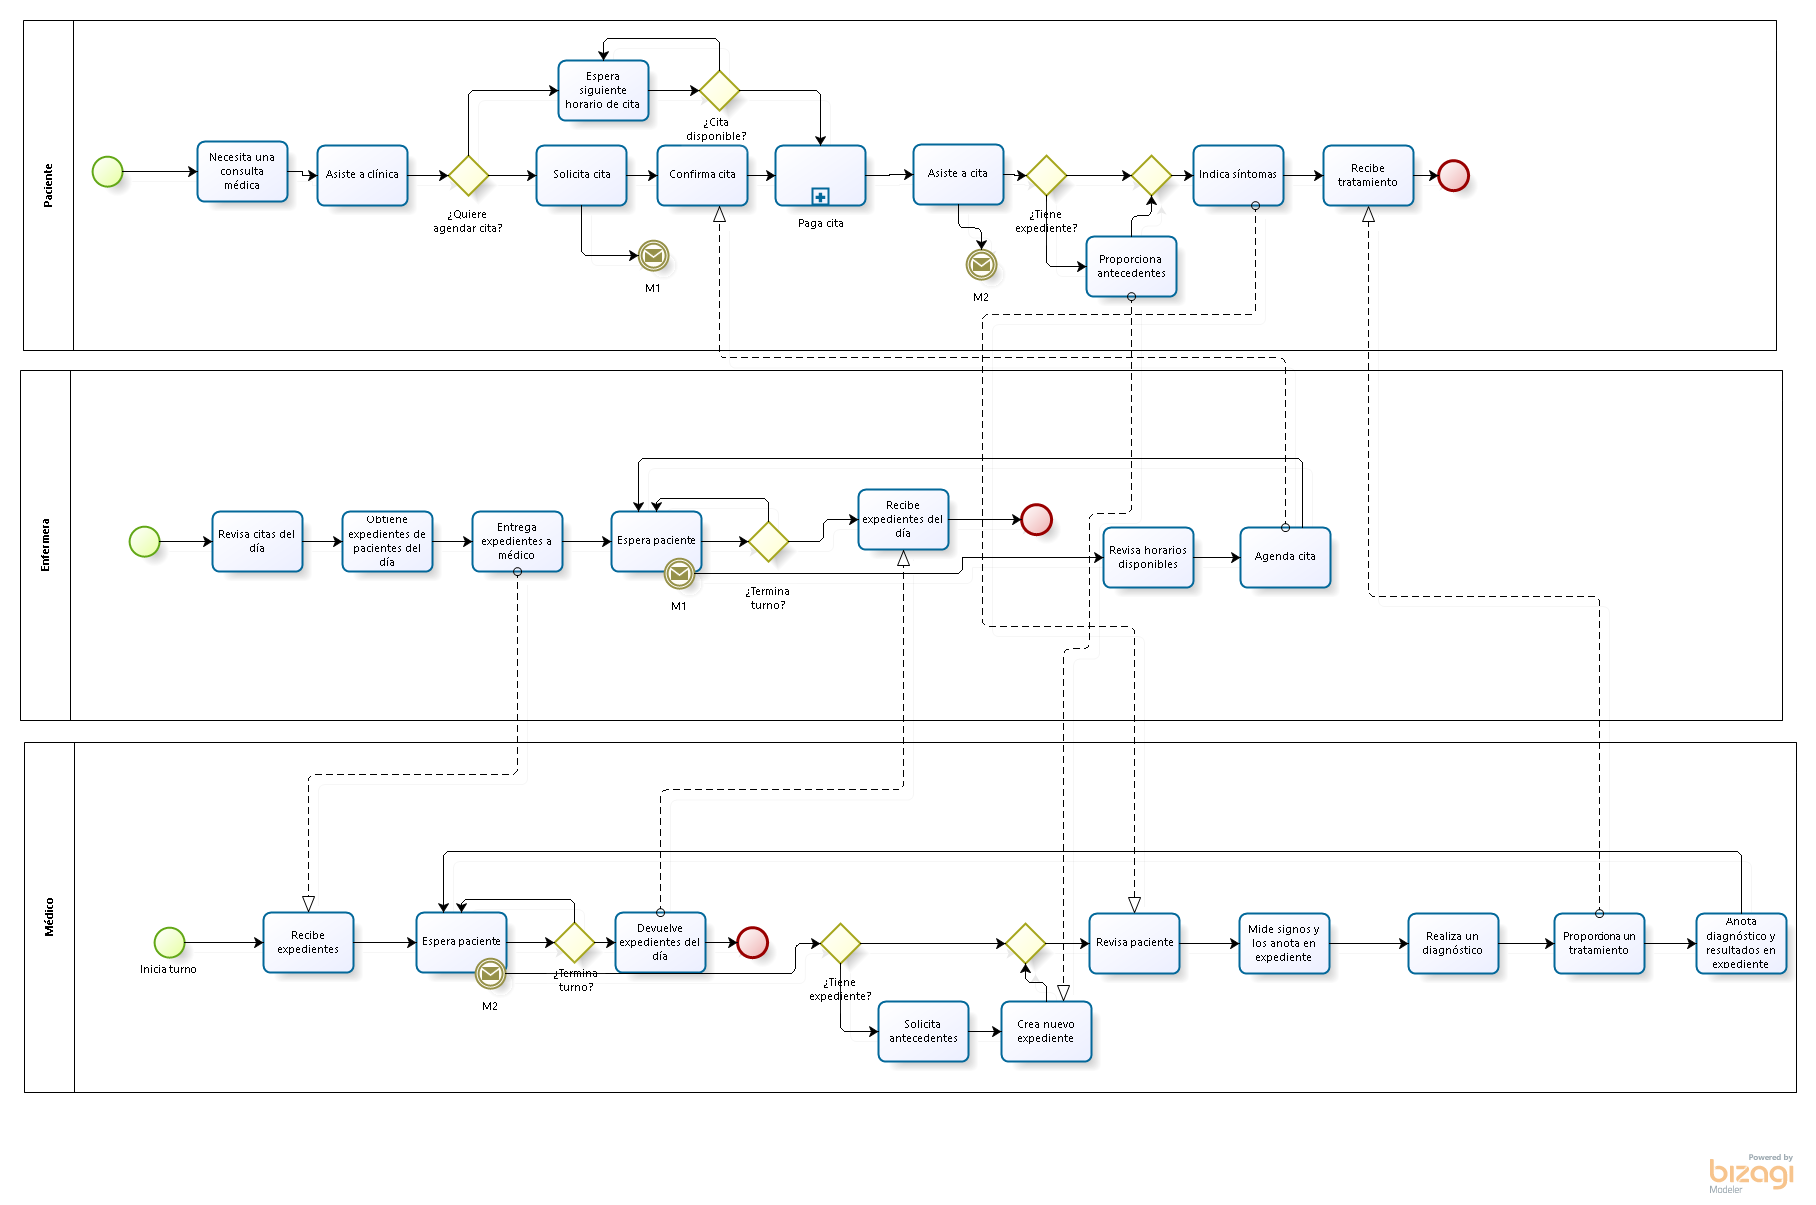
\includegraphics[width=\textwidth]{images/procesos/consultas_old}
	\caption{Diagrama del proceso actual para las consultas.}
\end{figure}
\paragraph{Paciente}
Cuando el paciente necesita una consulta médica, asiste a la clínica. Si quiere agendar una cita, lo solicita a la enfermera, confirma la cita. De otra manera espera el siguiente horario de cita. Posteriormente paga la cita en la caja, después asiste al consultorio, le indica sus síntomas al médico y en caso de que no tenga un expediente en la clínica, proporciona sus antecedentes médicos. Por último, recibe su tratamiento.
\paragraph{Enfermera}
Al iniciar su turno, revisa las citas agendadas para el día y obtiene los expedientes de los pacientes que asistirán a la clínica. Posteriormente entrega los expedientes de los pacientes que atenderán los médicos de la clínica. Durante el día se encargará de esperar a que lleguen los pacientes con citas agendadas. En caso de que llegue un paciente a agendar una cita revisa los horarios disponibles y agenda la cita. Finalmente, cuando termina su turno, recibe de los médicos los expedientes utilizados durante el día.
\paragraph{Médico}
Cuando inicia su turno, el médico recibe los expedientes de los pacientes que atenderá durante el día. En el transcurso del día, espera a que lleguen los pacientes con cita, cuando llega un paciente lo revisa. En caso de que el paciente no cuente con un expediente en la clínica, solicita sus antecedentes médicos y crea su expediente, después lo revisa. Al termina de revisar al paciente mide sus signos vitales y los anota en el expediente, posteriormente realiza su diagnóstico y proporciona un tratamiento al paciente, el cual anota en el expediente. Finalmente, cuando termina su turno, entrega a la enfermera los expedientes utilizados ese día.
\subsection{Cancelar cita}
\begin{figure}[htbp!]
	\centering
	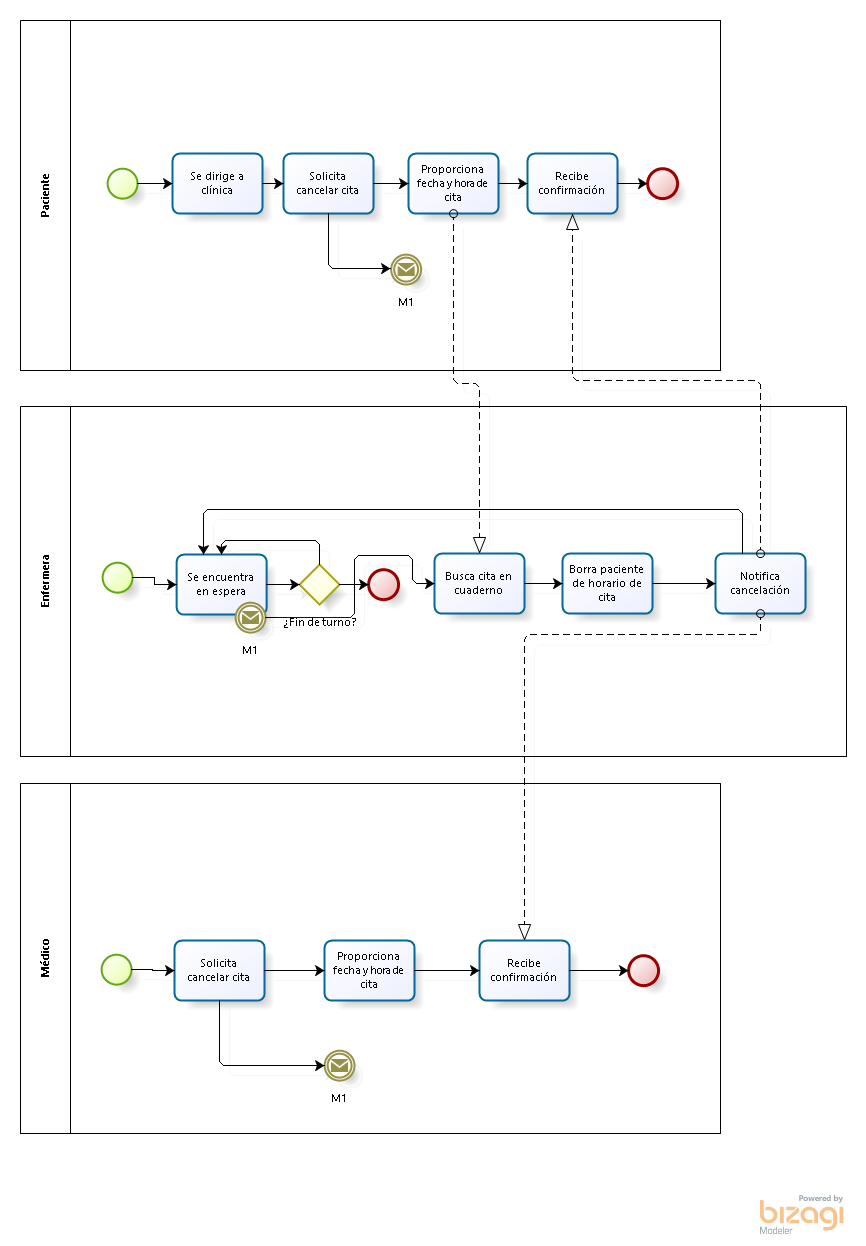
\includegraphics[width=\textwidth]{images/procesos/cancelar_cita_old}
	\caption{Diagrama del proceso actual para cancelar una cita.}
\end{figure}
\paragraph{Paciente}
Se dirige a la clínica, solicita cancelar su cita a la enfermera, después proporciona la fecha y hora de la cita que desea cancelar. Por último recibe una confirmación por parte de la enfermera.
\paragraph{Enfermera}
Durante su turno espera a que un paciente o un médico solicite cancelar una cita, una vez que llega el paciente busca la cita en el cuaderno. Cuando encuentra la cita borra al paciente del cuaderno de citas y le notifica la cancelación.
\paragraph{Médico}
Solicita cancelar una cita, después proporciona a la enfermera la fecha y hora de la cita que va a cancelar. Posteriormente recibe la confirmación de la cita cancelada.

\subsection{Pagar cita}
\begin{figure}[htbp!]
	\centering
	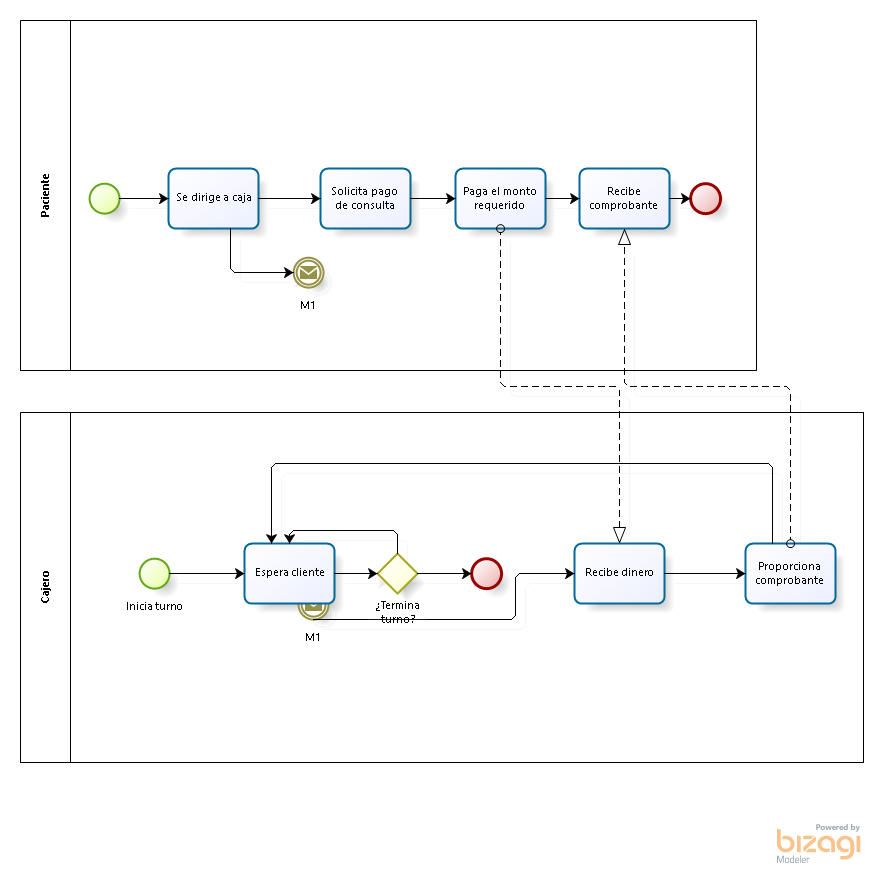
\includegraphics[width=\textwidth]{images/procesos/pago_consulta_old}
	\caption{Diagrama del proceso actual para cancelar una cita.}
\end{figure}
\paragraph{Paciente}
Se dirige a la caja, después solicita pagar una consulta. Posteriormente paga el monto de la consulta y el cajero le proporciona su comprobante de pago.
\paragraph{Cajero}
Mientras está en turno, espera a que llegue algún cliente, cuando esto pasa, recibe el dinero por el pago de la consulta y le proporciona el comprobante de pago al cliente.
\subsection{Comprar medicamentos}
\begin{figure}[htbp!]
	\centering
	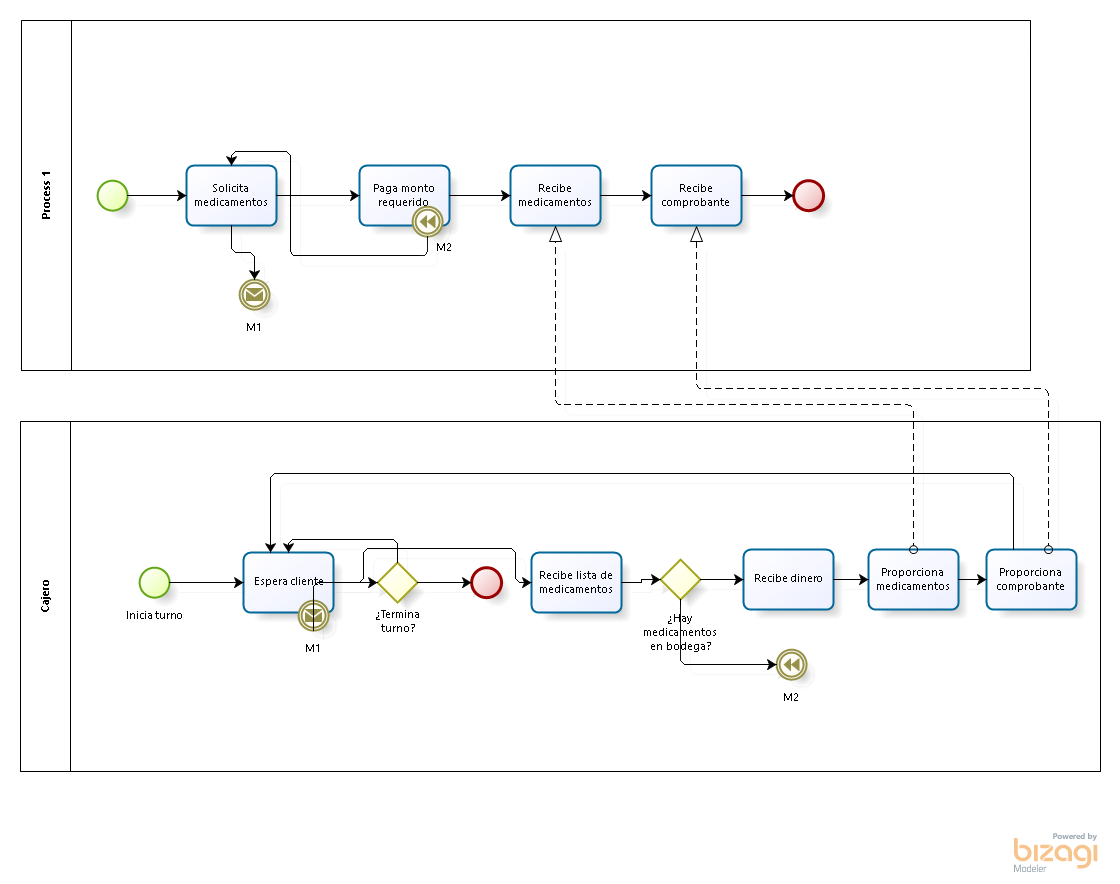
\includegraphics[width=\textwidth]{images/procesos/medicamentos_old}
	\caption{Diagrama del proceso actual para cancelar una cita.}
\end{figure}
\paragraph{Cliente}
Al comprar medicamentos en la farmacia, solicita los medicamentos requeridos, si estos se ecuentran disponibles en inventario paga el monto requerido. Finalmente recibe los medicamentos comprados y el comprobante de pago.
\paragraph{Cajero}
En el transcurso de su turno espera a que llegue un cliente a comprar medicamentos, cuando este llega, recibe la lista de los medicamentos; posteriormente valida si están todos los medicamentos de la lista disponibles en bodega, en caso de que no exista algún medicamento en bodega, le notifica al cliente. En caso afirmativo, recibe el dinero del costo de los medicamentos. Finalmente proporciona los medicamentos al cliente y el comprobante de pago.
    \newpage
